\documentclass{article}
\usepackage{color}
\usepackage{listings}
\usepackage{graphicx}
\usepackage{caption}
\usepackage{subcaption}
\usepackage{cite}

\lstset{ %
language=java,                % choose the language of the code
basicstyle=\footnotesize,       % the size of the fonts that are used for the code
numbers=left,                   % where to put the line-numbers
numberstyle=\footnotesize,      % the size of the fonts that are used for the line-numbers
stepnumber=1,                   % the step between two line-numbers. If it is 1 each line will be numbered
numbersep=5pt,                  % how far the line-numbers are from the code
backgroundcolor=\color{white},  % choose the background color. You must add \usepackage{color}
showspaces=false,               % show spaces adding particular underscores
showstringspaces=false,         % underline spaces within strings
showtabs=false,                 % show tabs within strings adding particular underscores
frame=single,           % adds a frame around the code
tabsize=2,          % sets default tabsize to 2 spaces
captionpos=b,           % sets the caption-position to bottom
breaklines=true,        % sets automatic line breaking
breakatwhitespace=false,    % sets if automatic breaks should only happen at whitespace
escapeinside={\%*}{*}          % if you want to add a comment within your code
}
\begin{document}
\tableofcontents{}


\newpage
\section{Einführung}
Die Performanz spielt eine große Rolle in der Entwicklung von Hardware und Software. Um herauszufinden ob gewisse Systeme eine bessere Rechenleistung besitzen als andere Systeme, 
werden ihre Performanz mit bestimmter Software, genannt Benchmarks, getestet.
Mit ihnen kann man die Grenzen der Hardware oder auch Software testen. Ein Beispiel wo Software getestet wird, sind Virtuelle Maschinen. 
Hier werden die Grenzen von virtuelle CPUs oder des Hypervisor analysiert. \cite{9256518}
Ein weiter Bereich, wo Benchmarking genutzt wird, ist Cloud Computing \cite{10.1145/2493123.2462919}. Somit gibt es ein weites Spektrum an Auswahl, wo solche Benchmarks verwendet werden.
Solche Grenzen könnte die Hardware, z.B CPU-Taktrate oder Brandbreitengeschwindigkeit beim Lesen oder Schreiben, aber auch Software (Komplexität von Algorithmen) sein. 


%\textit{Es werden daher standardisierten Benchmarks verwendet. Mit denen ist es möglich die Performanz verschiedener Hardware- und
%Softwareanbieter zu vergleichen.}

In Großkonzernen sind oft Performanzprobleme die eigentlichen Hindernisse, und nicht die funktionellen Probleme. Service Ausfälle sind höchst kostspielig. 
Aus diesem Grund werden solche Benchmarks in High Performance Computing (HPC) durchgeführt, um ihre Grenzen zu analysieren \cite{whenStopPerformanceTest}.
Ein Beispiel Programm für so ein Benchmark Tool ist das axboe/fio (flexible I/O tester) \cite{axboe2021github}.
In meiner Arbeit werde ich mit dem fio Tool arbeiten, um solche Performanz Änderungen zu berechnen und zu analysieren.
Fio ist ein Tool mit der man die Brandbreitengeschwindigkeit vom Lesen/Schreiben testen kann. Diese Tests lassen sich als eine Logdatei ausgeben.
Mein Programm wird mit diesen Logs arbeiten, um sie darstellen und analysieren zu können. Da diese Dateien zehntausende von Zeilen besitzen können.
Das Ziel soll es sein, dass man den stationären Zustand berechnet. \cite{baseline}

\section{Grundlagen}
Das Fio Tool ermöglicht das Testen auf bestimmter Hardware oder Software. Die I/O Geschwindigkeit wird hier in KiByte pro Sekunde angegeben.
Fio selbst besitzt kein GUI sondern arbeitet nur in der Konsole. Man kann für das Programm sogenannte .fio Dateien schreiben oder auch nur in der Konsole arbeiten,
um seine gewünschten Tests durchzuführen, wie z.B. ein random Read auf einer Datei.
Wenn man nun ein Random Read testen möchte, kann die .fio Datei wie folgt aussehen:
\bigskip
\begin{lstlisting}
    ; fio-rand-read.job for fio Test

    [global]
    name=rand-read # Name des Jobs
    rw=randread # Was soll der Job testen, randread = random read
    runtime=2s # Wie lange soll der Job laufen
    size=128m # Groesse der Datei, m fuer Megabyte
    write_bw_log=mytest # Name der Log-Datei
\end{lstlisting}
\bigskip
In der Konsole kann man sie auch einzeln als Parameter angeben, wenn es nur ein Test sein soll.
Zusätzlich können die Tests, oder auch Jobs genannt, Logs ausgeben, mit denen mein Tool arbeiten wird. Dieser Job oben testet das Random Read mit einer
maximalen Laufzeit (runtime) von 2 Sekunden und ließt eine Datei mit einer Größe von 2 Mebibyte. Mit größeren Tests ist es möglich den stationären Zustand zu analysieren. 
Der stationäre Zustand ist der Zeitpunkt, wenn es keine starken Schwankungen mehr bei der Brandbreitengeschwindigkeit im Lesen oder im Schreiben gibt.
Ein Hindernis bei dieser Analysierung könnten die nicht deterministischen Faktoren sein.
Auch wenn man Das Lesen/Schreiben auf dem selbem System mit der selben Datei testet, ist die Brandbreitengeschwindigkeit nie die gleiche, sondern sie schwankt immer. 
Ursachen dafür könnten schon verschiedene CPU Temperaturen sein, aber auch CPU Scaling oder parallele Prozessierung.
Da die Geschwindigkeit sich nie konstant einem Wert nähert sondern immer abweicht, soll mein Programm in Zukunft mithilfe der Standardabweichung den stationären Zustand ermitteln,
Solche Abweichung könnte in wenigen Prozentbereichen liegen. 

Es wird aber nicht ausreichen ein paar Tests durchzuführen und danach die Logs davon auszuwerten. Diese Logs wären nämlich nicht akkurat genug.
Man muss erst einige Warmup Iteration durchführen. Erst dann werden die Werte präziser \cite{baseline}. Somit hängt der stationäre Zustand
mit diesen Warmups zusammen. Dies sollte aber nur ein kleines Hindernis für mein Tool sein. Ein größeres Probleme könnte sein, wenn der Warmup durchgelaufen ist,
welche Logs am Ende die besten Information besitzen. \cite{whenStopPerformanceTest}

%Die Geschwindigkeit der Brandbreite ist abhängig von der CPU und des Speichermediums, wie SATA HDD, SATA SSD oder NVMe.
%The main data created by our experiment is the time taken by each in-process iteration to run.
%Formally, this is time series data of length 2000. In this Section we explain how we use statistical
%changepoint analysis to enable us to understand this time series data and classify the results we
%see, giving the first automated method for identifying warmup.
%\textit{NVMe drives are expected to be widely adopted in datacenters}.
%Warmup iterations
%are intended to bring the JVM into a steady state (e.g., exe-
%cute all applicable just-in-time compilations).


\section{Konzept}
fio besitzt ein extra Parameter, um solche Workloads als log ausgeben zu können.
Workloads oder auch Jobs, sind die Performanz Tests die mit dem fio gemacht werden.
Für diese Workloads möchte man noch gerne wissen was eigentlich für Werte Zustande kamen.
Die Logdatei besitzt die Information. Sie besitzt die Information vom verlauf des Jobs in Millisekunden.
Die jeweils 5 Werte besitzen und mit Kommas getrennt sind.
Mit dem Parameter $write\_bw\_logs=[Dateiname]$, kriege ich diese Logdatei: 
\bigskip
\begin{lstlisting}
    Time,	Bandwidth,	data direction, Blocksize,	Offset
    0, 	    59782, 		0,		        4096,		0
\end{lstlisting}
\bigskip
Time für die Zeit in Millisekunden (ms) die verlaufen ist, Bandwidth für die Brandweite in KiByte/s
Dritter Wert für die Date direction ob gelesen (= 0) oder geschrieben (= 1) wurde ein Blocksize
und ein Offset. Die Logdaten selbst sind immens lang und nicht schön lesbar. Deshalb wurde schon ein kleines Tool in Python gebaut 
was diese Logdaten zu einem Graph umwandelt. 
Die Y-Achse ist die Brandbreitengeschwindigkeit und X-Achse ist die vergangene Zeit des jeweiligen Jobs.
Wenn man die Logdaten anschaut, sieht man, dass die Brandbreitengeschwindigkeit sich schneller innerhalb einer 1 ms ändert.
\\
\begin{lstlisting}
    Drei Zeilen aus der Logdatei
    [Time,	Bandwidth,	data direction, Blocksize,	Offset]
    23, 	    59782, 		0,		        4096,		0
    23, 	    43534, 		0,		        4096,		0
    23, 	    54364, 		0,		        4096,		0

    Erste beide Spalten     ->          X-Y-Koordinaten
    X: 23       Y: 59782    ->        X: 23.0     Y: 59782
    X: 23       Y: 43534    ->        X: 23.3     Y: 43534
    X: 23       Y: 54364    ->        X: 23.6     Y: 54364
\end{lstlisting}
\bigskip
Da man die Daten nicht verwerfen möchte, wurden Wiederholungen linear getrennt. 
Diese Veranschaulichung wurde auf meinem Rechner getestet mit dem
Command die oben erwähnt wurde. Die Logdatei wurde ausgewertet und hier als .svg Datei dargestellt:

\begin{figure}
    \centering
    \begin{subfigure}{.5\textwidth}
      \centering
      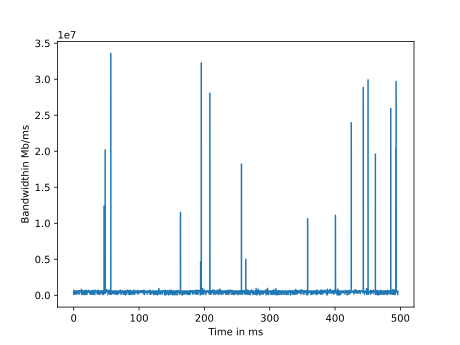
\includegraphics[width=1\linewidth]{./Code/nm_mytest_bw.jpg}
      \caption{A subfigure}
      \label{fig:sub1}
    \end{subfigure}%
    \begin{subfigure}{.5\textwidth}
      \centering
      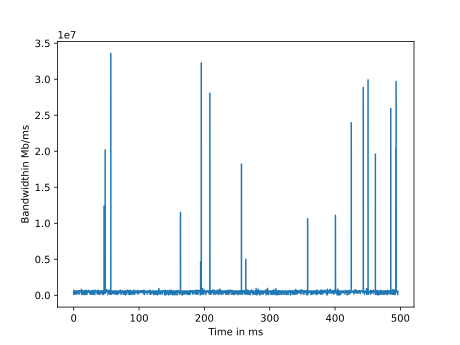
\includegraphics[width=1\linewidth]{./Code/nm_mytest_bw.jpg}
      \caption{A subfigure}
      \label{fig:sub2}
    \end{subfigure}
    \caption{A figure with two subfigures}
    \label{fig:test}
\end{figure}

Der Computer hat ein 11th Gen Intel(R) Core(TM) i5-11400 @ 2.60GHz und eine ADATA SWORDFISH SSD als Datenträger.
Es wurde ein kleines Tool geschrieben. Die eigentliche Arbeit wird es sein, das Tool weiter auszubauen das nicht nur veranschaulicht
sondern auch den stationären Zustand berechnet.
Nun erkennt man aber im Graph, dass diese Spikes zu sehen sind. Diese Spikes entstehen durch nicht deterministische Faktoren.
Das fio arbeitet nicht nur mit einem Thread, sondern es arbeitet Multithreaded, was zu nicht Determinismus führt. 
Das Programm wird in Java geschrieben. Grund dafür ist, da dort die bereits die meiste Erfahrung steckt.
Eine Möglichkeit, den stationären Zustand zu ermitteln, wäre das man die Standardabweichung verwendet und errechnet, wann die Abweichung klein ist.
Wann wurde der stationäre Zustand nun erreicht oder wann ist der Warmup fertig ? F-test,
which is used to test whether two variances are significantly different. Tukey HSD. Analysis of Variance (ANOVA). 
Mein Tool soll am Ende den stationären Zustand (z.B Warmup von VMs) berechnen können,
verschiedene Logs vergleichen können mit Hilfe der Standardabweichung, Varianz oder Tukey HSD

\textit{With improvements in storage device technology, the once negligible cost of I/O stack time has become more relevant (Foong et al. 2010; Caulfield et al. 2010). A number
of studies have provided proof of the I/O software stack being the major performance bottleneck in future storage systems.}
Im nächsten Graph werden die Häufigkeiten genommen für die Brandbreitengeschwindigkeit. X-Achse sind die Anzahl an Wiederholungen und Y-Achse die Geschwindigkeit.
\section{Verwandte Arbeiten}
Es wird auch auf nicht Determinismus von Computer, oder auch VMs, eingegangen \cite{vmsHotandCold}. Sie versucht man so gering wie möglich zu halten, da sonst bei der Auswertung nicht akkurate Werte
berechnet werden können. Nun lässt sich multithreading schlecht minimieren, da es dort meist Random verläuft, aber einige Methoden gibt es. Man kann, bei VMs,
erst sie erst mal warm laufen lassen \cite{vmsHotandCold}. Oder man versucht statistisch Methoden und arbeitet mit der Standardabweichung oder Konfident-werten
Das Tool, was entwickelt werden soll, wird mit solchen Methoden arbeiten. Die Methodiken oder statistischen Herangehensweisen die genommen werden,
stammen aus verschieden Arbeiten. Wann wird ein warmup erfolgt sein \cite{vmsHotandCold}
oder wann der stationären Zustand erreicht wurde \cite{vmsHotandCold}. Dabei soll das Tool nicht für spezifische Hardware dienen und wird zur reinen Analyse von fio Daten dienen. 
Dies ist von dem fio Tool abhängig.
Another source of non-determinism comes from thread scheduling in time-shared and multiprocessor systems. Running multithreaded
workloads, as is the case for most Java programs, requires thread scheduling in the operating system and/or virtual machine.  
\newpage
\section{Zeitplan}
\subsection{Einführung}
 \begin{itemize}
    \item Software und Performanz Bedeutung
    \item Benchmarks
    \item VMs, Cloud Computing
    \item Brandbreitengeschwindigkeit
    \item Probleme schlechter Performanz
    \item fio von axboe
    \item Mein Tool
    \item Allgemeines Ziel
 \end{itemize}
\subsection{Grundlagen}
\begin{itemize}
    \item Erklärung fio
    \item Ausführung fio
    \item .fio Datei
    \item fio in der Konsole
    \item Logs und Jobs
    \item Non-determinism
    \item stationärer Zustand
    \item Standardabweichung
\end{itemize}
\section{Exposee Notiz}
\subsection{Konzept}
\begin{itemize}
    \item Tool mit den Eigenschaften:
    \item Non-determinism
    \item stationärer Zustand
    \item Standardabweichung
    \item Varianz
    \item (Tukey HSD)
    \item Warmup VMs
    \item Sums of Squares (SSA)
\end{itemize}
\bibliography{cite}{}
\bibliographystyle{plain}
\end{document}